Upon the submission of a user defined trip, the CSA communicates with the SSA in order to produce a solution to it. This communication relies on HTTP, and utilizes the SSA API protocol that will be described in subsection \ref{sec:api_protocol}. The URL extension of the request, called the Uniform Resource Identifier (URI), enables the specification of each particular resource under request. Thus, the URI may be composed of the necessary fields that specify the attributes which characterize the user selected resource. It follows that a particular resource is identified by a collection of (key, value) pairs, which identify the resource attribute and its user defined value.

Although the application logic of the developed CSA is managed by Redux, this framework is not able to make HTTP requests or provide the desired asynchronous behaviour. In order to do so, it is necessary to use two third-party  libraries: redux-thunk and superagent. \textit{Redux-thunk} is a store enhancer, or a middleware, providing additional functionalities to the store: and \textit{superagent} is a library for \ac{AJAX} requests. Together, these two libraries enable the dispatch of asynchronous actions, which are used to make HTTP requests for specific resources to the SSA API.

%While Redux forces an action to return a pure JavaScript object, Redux-thunk overwrites this behaviour, allowing an action to return a function instead. This allows actions to dispatch other actions, updating the state multiple times in different moments. An asynchronous action may update the state twice: the first when the action is dispatched, and a second time when the request is complete. In order to inform the user that the request is being processed, the first action should update the state with some waiting information, while the secondary action interacts with the API.

%The details of the asynchronous action previously explained are illustrated in figure \ref{fig:ajax_request}. Note that an asynchronous request starts with an user defined action, dispatched from inside a component, and updates the Redux store at two particular moments in time: the first immediately, and the second after receiving the asynchronous response.

%\begin{figure}[htpb]
%  \centering
%  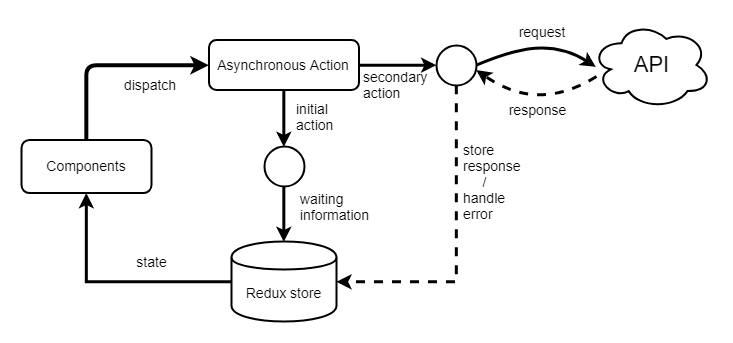
\includegraphics[width=\textwidth]{./Figures/system_implementation/async_request.png}
%  \caption{Asynchronous JavaScript request.}
%  \label{fig:ajax_request}  
%\end{figure}

